\chapter{Countermeasures Implementations}
\chaptermark{Countermeasures Implementations}
\label{chapter:countermeasures}
\minitoc

%%%%%%%%%%%%%%%%%%%%%%%%%%%%%%%%%%%%%%%%%%%%%%%%%%%%%%%%%%%%%%%%%%%%%%%%%%%%%%%%%%%%%%%%%%%%%%%
\section{Introduction}
Previous chapters have shown that the D-RI5CY's DIFT security mechanism is vulnerable to FIAs, mainly due to single-bit flips. This D-RI5CY essentially uses single-bit registers, as its data path is a single bit.

In this chapter, we present two countermeasures in order to protect the DIFT against fault injection attacks, and bit-flip.
The first countermeasure implemented to detect and prevent the use of corrupted data is simple parity. We selected the simple parity code as the error detection countermeasure because of its suitability and limited overhead.
The second countermeasure is implemented to detect any single-bit errors that may occur, but also to correct them without time overhead. With this countermeasure, we want to correct to the nearest cycle so that the fault cannot propagate and give a potential attacker the impression that the fault he injected had no effect on the system.
This work has been published in ISVLSI 2024~\cite{PRLG-24-isvlsi}.

The first section of this chapter presents the different fault models considered. Then, the second section details the implementation of simple parity and briefly presents how it works. Afterwards, the third section presents the working of Hamming code, with a simple example, and details our implementation. Finally, we discuss these countermeasures and compare them.

%%%%%%%%%%%%%%%%%%%%%%%%%%%%%%%%%%%%%%%%%%%%%%%%%%%%%%%%%%%%%%%%%%%%%%%%%%%%%%%%%%%%%%%%%%%%%%%
\section{Fault models used in this chapter}
In Chapter~\ref{chapter:dift_assessment}, we assessed the D-RI5CY design by considering \textit{single bit-flip in one register at a given clock cycle}, \textit{bit reset}, and \textit{bit set} fault models. The conclusion of this chapter was that the D-RI5CY is vulnerable mostly to single bit-flip.

In this chapter, we consider an attacker able to inject faults into DIFT-related registers, leading to single bit-flips at any position of the targeted register. To reach this objective, any DIFT-related register maintaining 1-bit tag value, driving the tag propagation or the tag update process or maintaining the security policy configuration can be targeted. Studies presented in~\cite{ZDCRT-12-dcis,CLFT-14-cosade} have shown that such precise single bit-flip attacks targeting registers can be performed using, for example, laser shots. We also consider an attacker able to inject a \textit{single bit-flip in two registers at two distinct clock cycles}, with a minimum delay of one clock cycle.

%%%%%%%%%%%%%%%%%%%%%%%%%%%%%%%%%%%%%%%%%%%%%%%%%%%%%%%%%%%%%%%%%%%%%%%%%%%%%%%%%%%%%%%%%%%%%%%
\section{Countermeasure 1: Simple Parity}
\label{chapter:simpleparity}

Error detection is often achieved through the use of parity codes, which involve adding an extra bit to the data bits. Simple parity codes can detect single-bit errors. Simple parity can take into account odd parity or even parity, which means in case of an even parity, the number of bit set to '\texttt{1}' will be even with the message bits and parity bit.

%%%%%%%%%%%%%%%%%%%%%%%%%%%%%%
\subsection{Presentation of the simple parity}
Simple parity involves adding one bit to the data. This one bit store the parity of the initial message. Figure~\ref{fig:simpleparity_functionning} shows how the data, in blue, and the parity bit, in red, are associated to form an encoded data.

\begin{figure}[ht]
    \centering
    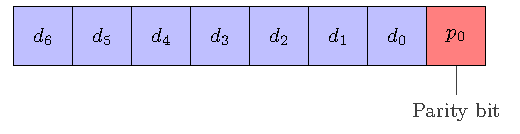
\includegraphics[page=1]{c5_countermeasures_dift/img/simple_parity.pdf}
    \caption{Simple Parity -- functioning}
    \label{fig:simpleparity_functionning}
\end{figure}

Equation~\ref{equat:simpleparity} shows how the parity bit is computed. Each bit of the initial message is XOR'd to show parity. Table~\ref{tab:xor_truthtable} present the truth table of XOR operations.

\begin{equation} \label{equat:simpleparity}
    \begin{split}
        p_{0} &= d_{0} \oplus d_{1} \oplus d_{2} \oplus d_{3} \oplus d_{4} \oplus d_{5} \oplus d_{6}
    \end{split}
\end{equation}

\begin{table}[t]
    \centering
    \footnotesize
    \caption{XOR truth table}
    \label{tab:xor_truthtable}
    \begin{tabular}{@{}c|c|c@{}}
        \toprule
        A & B & $A \oplus B$ \\\midrule
        0 & 0 & 0            \\
        0 & 1 & 1            \\
        1 & 0 & 1            \\
        1 & 1 & 0            \\
        \bottomrule
    \end{tabular}
\end{table}

Figures~\ref{fig:simpleparity_example_1} and \ref{fig:simpleparity_example_2} show an example of a message with its parity bit associated. The message is \texttt{0b1001101} in binary. Hence, as there is an even number of '\texttt{1}', the parity bit is set to '\texttt{0}' (cf Table~\ref{tab:xor_truthtable}).

\begin{figure}[ht]
    \centering
    \begin{subfigure}[b]{0.49\textwidth}
        \includegraphics[width=\textwidth, page=2]{c5_countermeasures_dift/img/simple_parity.pdf}
        \caption{Initial message}
        \label{fig:simpleparity_example_1}
    \end{subfigure}
    \hfill
    \begin{subfigure}[b]{0.49\textwidth}
        \includegraphics[width=\textwidth, page=3]{c5_countermeasures_dift/img/simple_parity.pdf}
        \caption{Message with its parity bit}
        \label{fig:simpleparity_example_2}
    \end{subfigure}
    \hfill
    \begin{subfigure}[b]{0.49\textwidth}
        \includegraphics[width=\textwidth, page=4]{c5_countermeasures_dift/img/simple_parity.pdf}
        \caption{Single-bit fault inside the message}
        \label{fig:simpleparity_faulted_example_3}
    \end{subfigure}
    \hfill
    \begin{subfigure}[b]{0.49\textwidth}
        \includegraphics[width=\textwidth, page=5]{c5_countermeasures_dift/img/simple_parity.pdf}
        \caption{Two single-bit faults inside the message}
        \label{fig:simpleparity_faulted_example_4}
    \end{subfigure}
    \caption{Example of a simple parity computation}
    \label{fig:simpleparity_example}
\end{figure}

Figures~\ref{fig:simpleparity_faulted_example_3} and \ref{fig:simpleparity_faulted_example_4} present, respectively, two examples of when a fault occur and when two faults happen.
In the first example, Figure~\ref{fig:simpleparity_faulted_example_3}, the bit $d_2$ is faulted. As the faulted message is \texttt{0b1001001}, it means that the parity bit will change from \texttt{0} to \texttt{1}. Hence, the fault will be detected as the parity bit differs from the original computed message (Figure~\ref{fig:simpleparity_example_2}).
In the second case, two faults happen in the message at bits $d_2$ and $d_5$. So, the faulted message is \texttt{0b1101001}, then, when the parity is computed, the parity bit will not change as there is still an even number of \texttt{1} compared to the initial message. This shows the limitation of this code.

%%%%%%%%%%%%%%%%%%%%%%%%%%%%%%
\subsection{Implementation: Optimisation of redundancy bits}

In order to implement simple parity, we decided to optimise the number of parity bits. We had many choices, but we decided to form five groups. These groups are composed of one or more register according to their criticality.
Firstly, the two registers that contain the security policy, TCR and TPR, are highly critical. As a result, we have chosen to form a separate group for each of them. Although these registers are 32 bits long, only 22 bits are fully utilised in the current implementation, making bits 22 to 31 unnecessary. Therefore, we have decided not to protect these unused bits or include them in parity calculations.
Secondly, the third logical group consists of keeping the 32 registers of the register file tag together. Since these registers are already grouped, it makes sense to maintain this grouping.
This leaves us with one 5-bit register, sixteen 1-bit registers, three 2-bit registers, and one 4-bit register. The 5-bit register is used to store the tag destination address, which is critical. As such, we have decided to create a dedicated group for it. The remaining 20 registers, which total 26 bits, are combined into a fifth group.
Table~\ref{tab:sp_group} shows the five groups formed to implement the protection for 107 bits in total. Each group is protected by one parity bit.

\begin{table}[t]
    \centering
    \small
    \caption{DIFT-related protected registers -- simple parity}
    \label{tab:sp_group}
    \begin{tabular}{@{}ccccc@{}}
        \toprule
                & Protected register                                                                                & \begin{tabular}[c]{@{}c@{}}Number of\\ bits\end{tabular} & \begin{tabular}[c]{@{}c@{}}Number of\\ protected bits\end{tabular} & \begin{tabular}[c]{@{}c@{}}Number of\\ parity bits\end{tabular} \\ \midrule
        Group 1 & TCR                                                                                               & 32                                                       & 22                                                                 & 1                                                               \\
        Group 2 & TPR                                                                                               & 32                                                       & 22                                                                 & 1                                                               \\
        Group 3 & Register File (Tag)                                                                               & 32                                                       & 32                                                                 & 1                                                               \\
        Group 4 & Tag destination address                                                                           & 5                                                        & 5                                                                  & 1                                                               \\
        Group 5 & \begin{tabular}[c]{@{}c@{}}16×1-bit registers\\ 3×2-bit registers\\ 1×4-bit register\end{tabular} & 26                                                       & 26                                                                 & 1                                                               \\ \midrule
        Total   &                                                                                                   & 127                                                      & 107                                                                & 5                                                               \\
        \bottomrule
    \end{tabular}
\end{table}

Figure~\ref{fig:implementation_sp} presents our proposed implementation for the simple parity. This implementation is simple. In order to protect a register, it takes its input and send its input into both the protected register and an encoder.

\begin{figure}[ht]
    \centering
    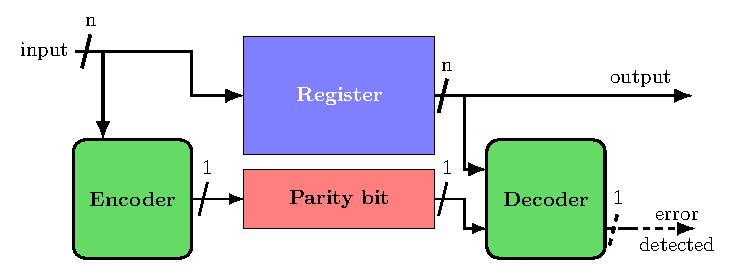
\includegraphics[page=1]{c5_countermeasures_dift/img/archi_contremesures.pdf}
    \caption{Implementation of simple parity}
    \label{fig:implementation_sp}
\end{figure}


%%%%%%%%%%%%%%%%%%%%%%%%%%%%%%%%%%%%%%%%%%%%%%%%%%%%%%%%%%%%%%%%%%%%%%%%%%%%%%%%%%%%%%%%%%%%%%%
\section{Countermeasure 2: Hamming Code}
\label{chapter:hammingcode}

%%%%%%%%%%%%%%%%%%%%%%%%%%%%%%
\subsection{Presentation of Hamming Code}
~\cite{H-50-bstj}

\begin{figure}[ht]
    \centering
    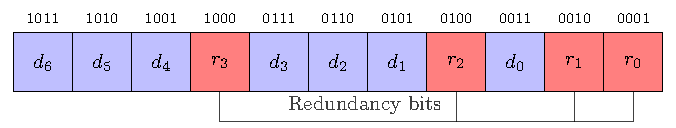
\includegraphics[page=1]{c5_countermeasures_dift/img/hamming_bit.pdf}
    \caption{Hamming code -- functioning}
    \label{fig:hamming_functionning}
\end{figure}

\begin{equation} \label{equat:hamming_encoder}
    \begin{split}
        r_{0} &= d_{0} \oplus d_{1} \oplus d_{3} \oplus d_{4} \oplus d_{6} \\
        r_{1} &= d_{0} \oplus d_{2} \oplus d_{3} \oplus d_{5} \oplus d_{6} \\
        r_{2} &= d_{1} \oplus d_{2} \oplus d_{3} \\
        r_{3} &= d_{4} \oplus d_{5} \oplus d_{6}
    \end{split}
\end{equation}

%%%%%%%%%%%%%%%%%%%%%%%%%%%%%%
\subsection{Implementation 1: Optimisation of redundancy bits}

\begin{table}[t]
    \centering
    \small
    \caption{DIFT-related protected registers -- Hamming code}
    \label{tab:hammingcode_group}
    \begin{tabular}{@{}ccccc@{}}
        \toprule
                & Protected register                                                                                & \begin{tabular}[c]{@{}c@{}}Number of\\ bits\end{tabular} & \begin{tabular}[c]{@{}c@{}}Number of\\ protected bits\end{tabular} & \begin{tabular}[c]{@{}c@{}}Number of\\ redundancy bits\end{tabular} \\ \midrule
        Group 1 & TCR                                                                                               & 32                                                       & 22  & 5                                                                                                               \\
        Group 2 & TPR                                                                                               & 32                                                       & 22  & 5                                                                                                               \\
        Group 3 & Register File (Tag)                                                                               & 32                                                       & 32  & 6                                                                                                               \\
        Group 4 & Tag destination address                                                                           & 5                                                        & 5   & 4                                                                                                               \\
        Group 5 & \begin{tabular}[c]{@{}c@{}}16×1-bit registers\\ 3×2-bit registers\\ 1×4-bit register\end{tabular} & 26                                                       & 26  & 5                                                                                                               \\ \midrule
        Total   &                                                                                                   & 127                                                      & 107 & 25                                                                                                              \\
        \bottomrule
    \end{tabular}
\end{table}

\begin{figure}[ht]
    \centering
    \includegraphics[page=2, width=\textwidth]{c5_countermeasures_dift/img/archi_contremesures.pdf}
    \caption{Implementation of Hamming Code}
    \label{fig:implementation_hc_1}
\end{figure}

\begin{figure}[ht]
    \centering
    \includegraphics[page=3, width=\textwidth]{c5_countermeasures_dift/img/archi_contremesures.pdf}
    \caption{Implementation of Hamming Code -- Register Tile Tag}
    \label{fig:implementation_hc_2}
\end{figure}

%%%%%%%%%%%%%%%%%%%%%%%%%%%%%%%%%%%%%%%%%%%%%%%%%%%%%%%%%%%%%%%%%%%%%%%%%%%%%%%%%%%%%%%%%%%%%%%
\section{Evaluation and discussion}


\begin{table}[t]
    \footnotesize
    \centering
    \caption{Logical fault injection simulation campaigns results for single bit-flip in one register at a given clock cycle}
    \label{tab:chap5_results_single_bitflip}
    \setlength{\tabcolsep}{3pt}
    \begin{tabular}{@{}ccccccccc@{}}
        \toprule
                                           &               & Crash & Silent & Delay & Detection & \begin{tabular}[c]{@{}c@{}}Detection \&\\ Correction\end{tabular} & Success     & Total \\ \midrule
        \multirow{3}{*}{Buffer overflow}   & No protection & 0     & 738    & 12    & —         & —                       & 12 (1.57\%) & 762   \\
                                           & Simple parity & 0     & 0      & 0     & 792       & —                       & 0           & 792   \\
                                           & Hamming Code  & 0     & 0      & 0     & —         & 912                     & 0           & 912   \\\midrule
        \multirow{3}{*}{Format String}     & No protection & 0     & 946    & 41    & —         & —                       & 29 (2.85\%) & 1,016 \\
                                           & Simple parity & 0     & 0      & 0     & 1,056     & —                       & 0           & 1,056 \\
                                           & Hamming Code  & 0     & 0      & 0     & —         & 1,216                   & 0           & 1,216 \\\midrule
        \multirow{3}{*}{Compare / Compute} & No protection & 0     & 491    & 7     & —         & —                       & 10          & 508   \\
                                           & Simple parity & 0     &        &       &           & —                       &             &       \\
                                           & Hamming Code  & 0     &        &       & —         &                         &             &       \\
        \bottomrule
    \end{tabular}
\end{table}

\begin{table}[t]
    \footnotesize
    \centering
    \caption{Logical fault injection simulation campaigns results for single bit-flip in two registers at two clock cycles}
    \label{tab:chap5_results_tempo}
    \setlength{\tabcolsep}{3pt}
    \begin{tabular}{@{}ccccccccc@{}}
        \toprule
                                           &               & Crash & Silent  & Delay  & Detection & \begin{tabular}[c]{@{}c@{}}Detection \&\\ Correction\end{tabular} & Success         & Total   \\ \midrule
        \multirow{3}{*}{Buffer overflow}   & No protection & 0     & 238,633 & 1,143  & —         & —                       & 2,159 (0.89\%)  & 241,935 \\
                                           & Simple parity & 0     & 0       & 0      & 261,360   & —                       & 0               & 261,360 \\
                                           & Hamming Code  & 0     & 0       & 0      & —         & 346,560                 & 0               & 346,560 \\\midrule
        \multirow{3}{*}{Format String}     & No protection & 0     & 429,260 & 12,192 & —         & —                       & 10,160 (2.25\%) & 451,612 \\
                                           & Simple parity & 0     & 0       & 0      & 487,872   & —                       & 0               & 487,872 \\
                                           & Hamming Code  & 0     & 0       & 0      & —         & 646,912                 & 0               & 646,912 \\\midrule
        \multirow{3}{*}{Compare / Compute} & No protection & 0     & 491     & 7      & —         & —                       & 10              & 508     \\
                                           & Simple parity & 0     &         &        &           & —                       &                 &         \\
                                           & Hamming Code  & 0     &         &        & —         &                         &                 &         \\
        \bottomrule
    \end{tabular}
\end{table}

%%%%%%%%%%%%%%%%%%%%%%%%%%%%%%%%%%%%%%%%%%%%%%%%%%%%%%%%%%%%%%%%%%%%%%%%%%%%%%%%%%%%%%%%%%%%%%%
\section{Summary}

%%%%%%%%%%%%%%%%%%%%%%%%%%%%%%%%%%%%%%%%%%%%%%%%%%%%%%%%%%%%%%%%%%%%%%%%%%%%%%%%%%%%%%%%%%%%%%%